

\documentclass[12pt]{article}
\usepackage{graphicx}
\usepackage{float} 
\usepackage{amsmath}
\usepackage{listings}
\usepackage{color}

\definecolor{dkgreen}{rgb}{0,0.6,0}
\definecolor{dkblue}{rgb}{0,0.0,0.6}
\definecolor{dkred}{rgb}{0.9,0.0,0.1}


\begin{document}

\lstset{language=Fortran,tabsize=4,numbers=left,numberstyle=\tiny,basicstyle=\ttfamily\small\color{dkblue},stringstyle=\ttfamily\color{blue},keywordstyle=\rmfamily\color{dkred}\bfseries\emph,backgroundcolor=\color{white},commentstyle=\color{dkgreen}}




\title{Blackbody Radiation at Specific Temperatures}
\author{Benjamin Deutsch  \\
Department of Physics\\
California State University Long Beach}
\date{\today }

  
\maketitle



\begin{abstract}
This report gives instruction and results on compiling Planck's Law on Blackbody Radiation in the Fortran Language.
\end{abstract}

\section{Introduction}

Blackbody radiation as described in physics subsumes that standard baryonic matter with a temperature above absolute zero will emit electromagnetic radiation. 
As a material becomes heated it converts its thermal energy to electromagnetic radiation, disassociating through entropy. The radiation emitted by the heated body, is charateristic only by the body its self and not the energy it is absorbing. The theory of blackbodies played an integral role in the understanding of quantum effects as the frequencies which are emitted are tied up in the resonant modes of the item. This is a universal effect extending to all areas and materials, however it should be noted that this concept is idealized in that the "blackbody" a form which absorbs all radiation falling into it, does not exist.

To explore this, we will make use of ideas and methods made available by the advanced computational physics seminar.
As scientists have incorporated new tools in modern research, we will make us of computers to help model the behaviors of these blackbodies. 

The experiment will been completed using a Mac computer running on OSX operating system, and modified by the faculty to operate as they deem helpful.

Programming will be done in XCode, utilizing the Fortran95 language with the GNU compiler, {\tt gfortran}.  
Text editing will be placed in Text Wrangler, all additions to the programming environment were placed for streamlining and their cost effective nature.



\section{The Math}

The exercise given for completion in the paper, was to investigate the  mechanics of Plancks Law of blackbody radiation. This set of equations takes variables in for temperature and frequency and produces a trending curve to express the radiation given off by the material. As this is well researched area, and as many experimental analogs, the goal is to produce a program which will agree with current reviewed data. The equation set is seen here in (1).


\begin{align}
		B(\nu,T)  = \frac{2h\nu^3}{c^2} n_{BE} (\nu,T), \hspace{5mm} with \hspace{5mm}   n_{BE} (\nu, T) \equiv  \frac {1}{e^\frac{h\nu}{k_B T}-1}
\end{align}
 

The code can be found in the {\tt .f95} included in the assignment package.
 
 \section{Description of code}


The key to coding the above referenced equations is to make use of the dimensionless units values in 


\begin{align} 
	n_{BE} (\nu, T) \equiv  \frac {1}{e^\frac{h\nu}{k_B T}-1}
\end{align}



Here we notice that the values; 



\begin{align}
	e^\frac{h\nu}{k_B T}  = EE,
\end{align}

Returning,

\begin{align}
	\frac{2h\nu^3}{c^2} \frac{1}{e^{EE}-1} = Eq(EE,T) 
\end{align} 

Solving and collecting constants 

\begin{align} 
(Constants)*\frac {EE^3}{e^{EE}-1} = Eq(EE,T) 
\end{align}

The end result can be placed in Fortran language more or less straightforwardly, in effect we have simply absorbed the variable "v" into EE to use in to calculation of the data curves.

This is transcribed very systematically in Fortran and can be seen mirrored in most of this languages program. Firstly, we have a section in which we need to declare variables, for reference to this code this exist has either constants, real double precisions variables (numbers contains decimals places) , or integers used for counting. Next and most importantly these variables are called into play with do loops, this is the actual computing level of the programs. The loops happen for a iterative amount of cycles, defined here in code as integer i = 0, 10000. We now have to make use of the integer that will be cycled, the {\tt{float}} function, inputs the integer {\tt{i}} value and allows for the output of a real numerically useful value. Different things can be done with the output, but for our code it is placed each cycled into the equations (5), to give the data point needed. With successive data points written for 10000+1 (starting at 0), we have chosen to print and write the information to a separate file for plotting which can be seen below in Section 4. Plotting was done in Plot2 Pro. This looping completes for each temperature called for by the do loop ; T1, T2, T3, (identified in the header)by the end do commend before moving on the next loop in series. 

\section {Results} 
\begin{figure}[H]
	\centering
	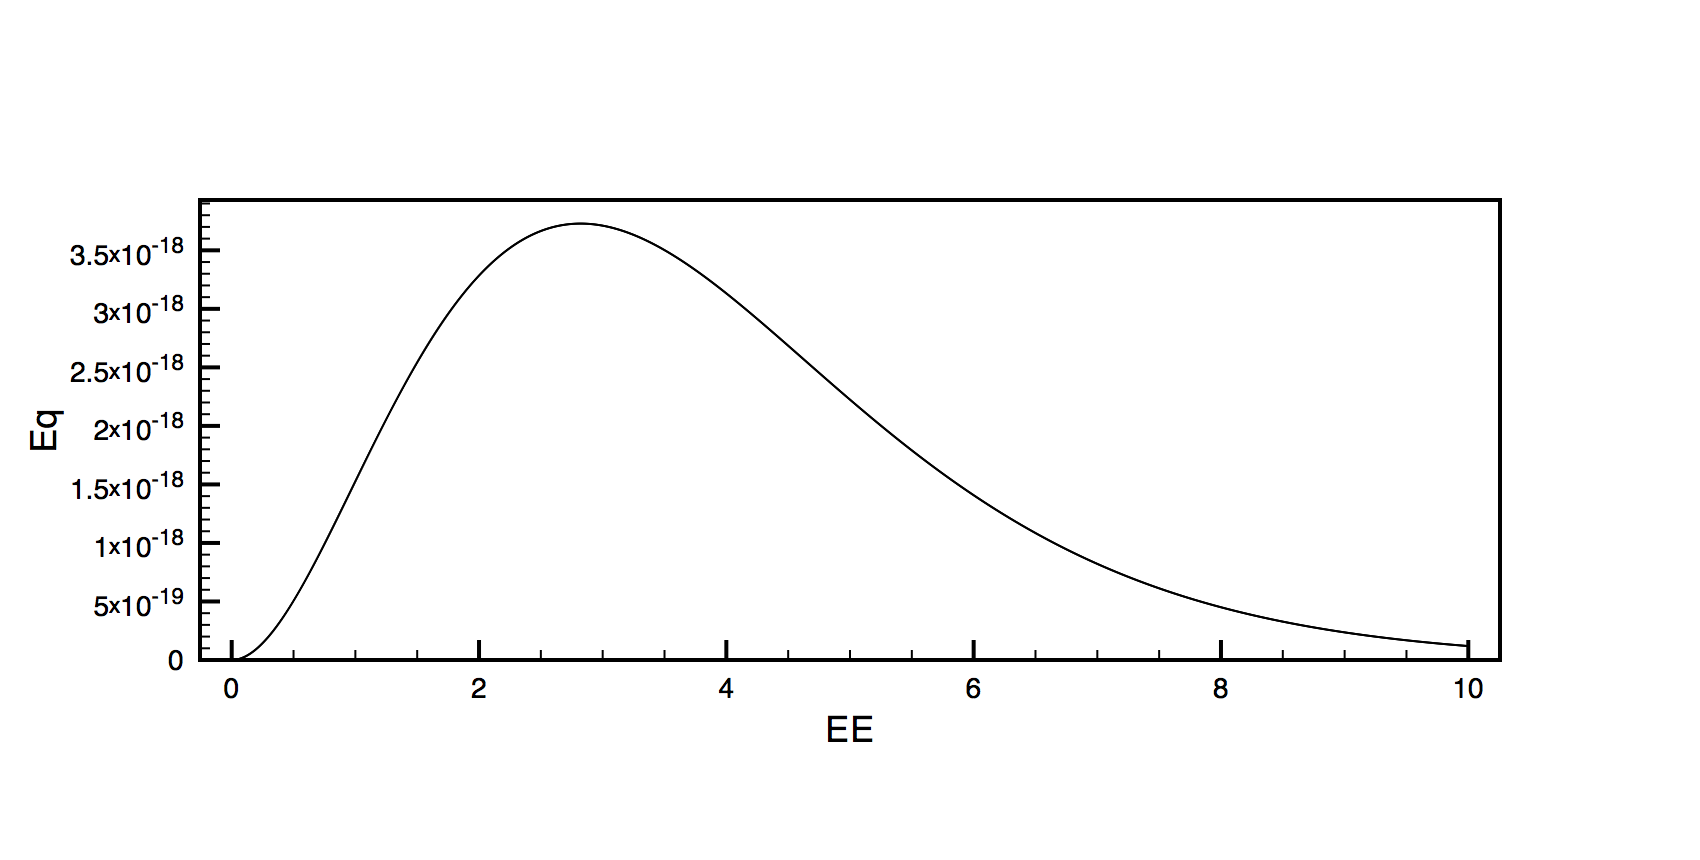
\includegraphics[width=1.\textwidth]{11.png}
	\caption{EE vs Eq at 2.7 Kelvin}
\end{figure}

\begin{figure}[H]
	\centering 
	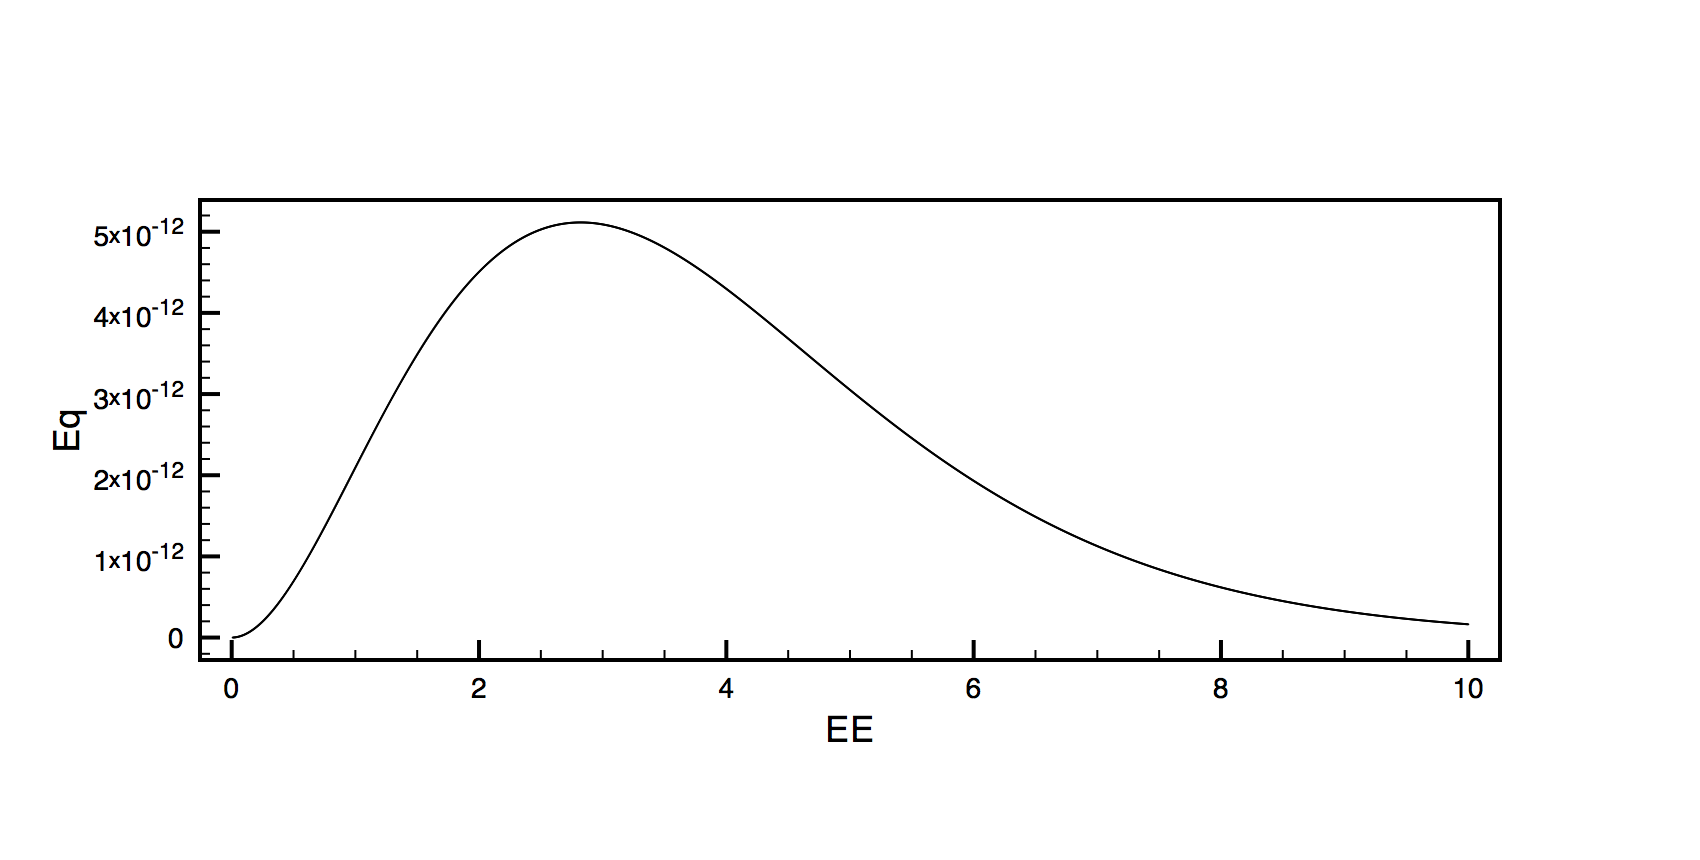
\includegraphics[width=1.\textwidth]{12.png}
	\caption{EE vs Eq at 300 Kelvin}
\end{figure}

\begin{figure}[H]
	\centering 
	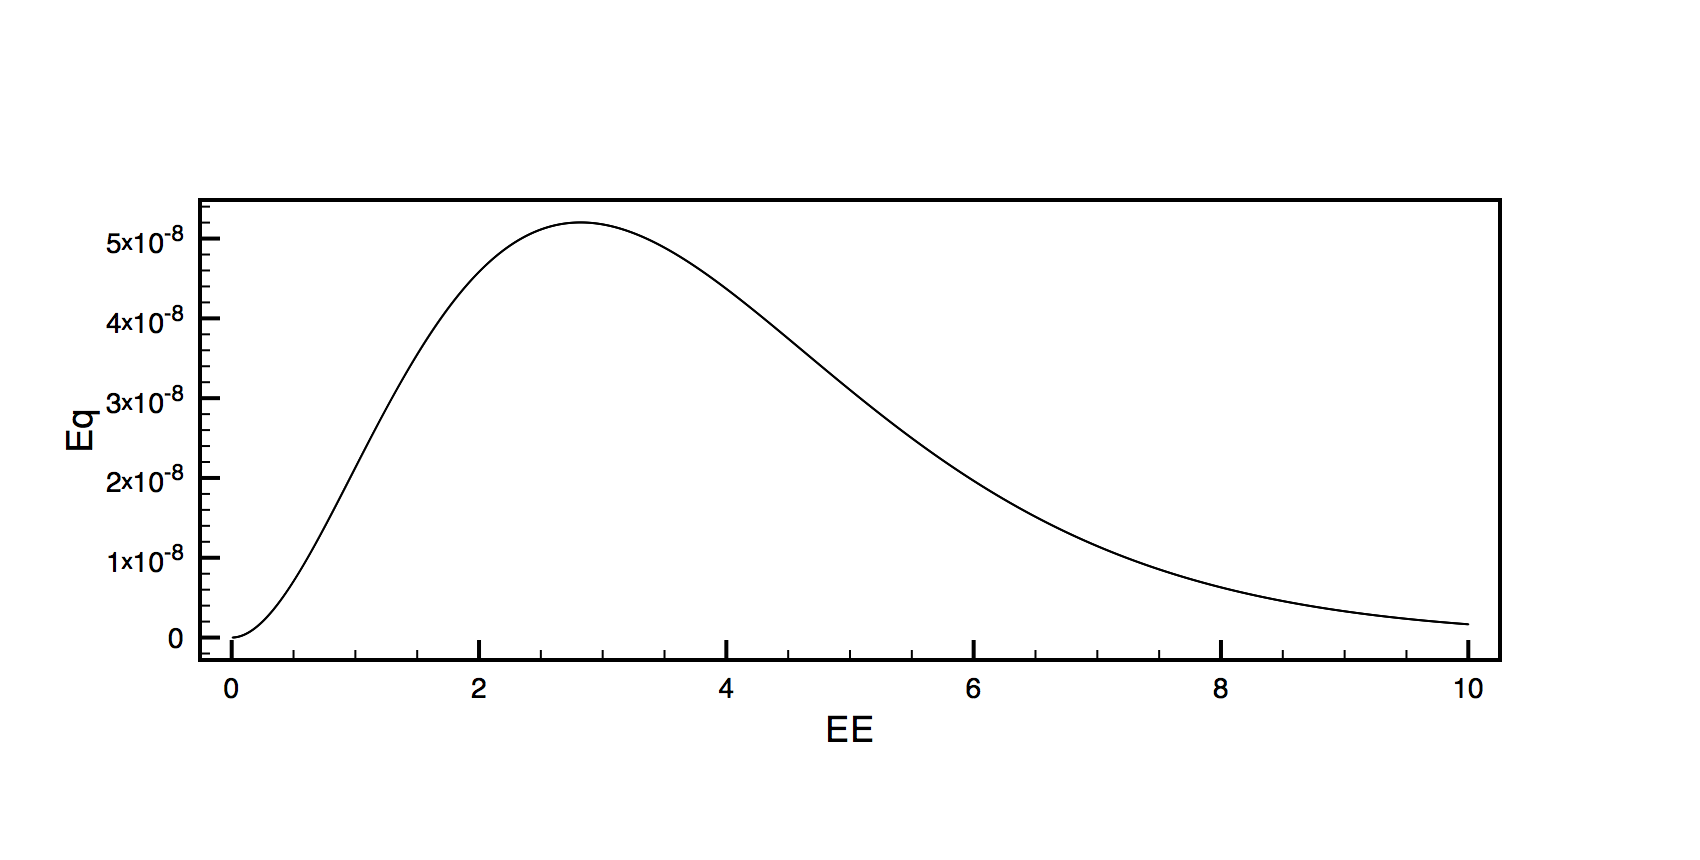
\includegraphics[width=1.\textwidth]{13.png}
	\caption{EE vs Eq at 6500 Kelvin}
\end{figure}

We can also simply return to the original  $\nu$ , frequency. 

\begin{align} 
\frac {K_B*T*EE}{h} = \nu 
\end{align}

As seen on the following page,

\begin{figure}[H]
	\centering 
	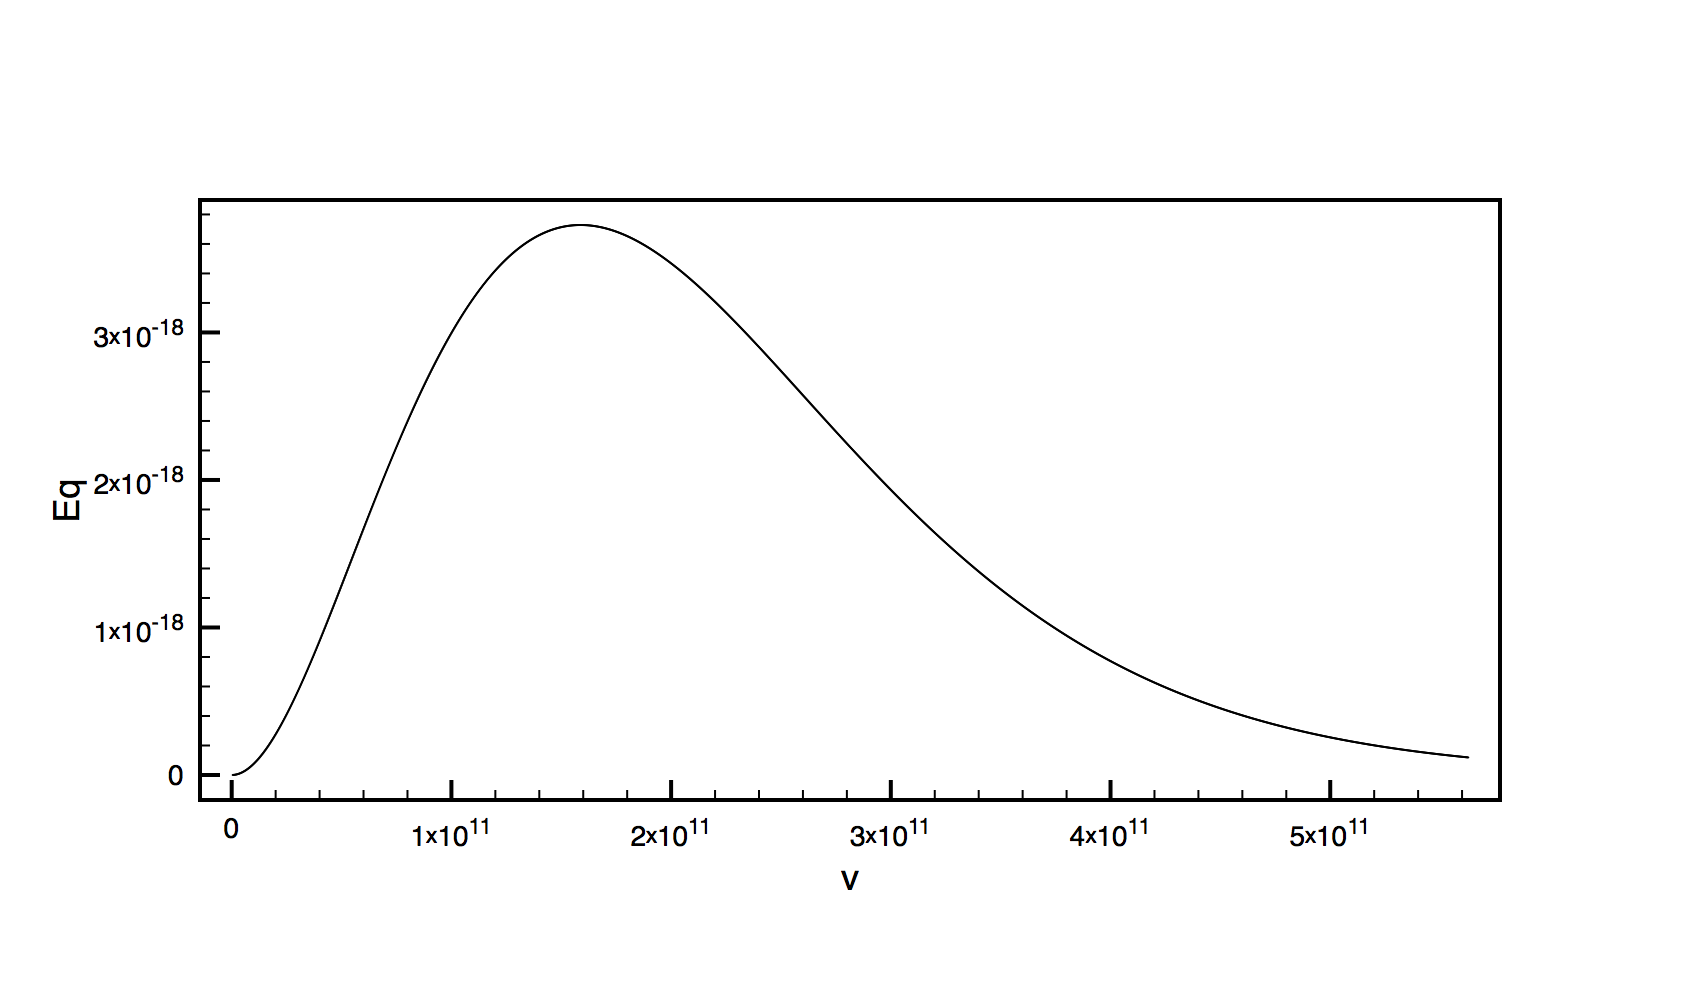
\includegraphics[width=1.\textwidth]{21.png}
	\caption{ V vs Eq at 2.7 Kelvin}
\end{figure}

\begin{figure}[H]
	\centering 
	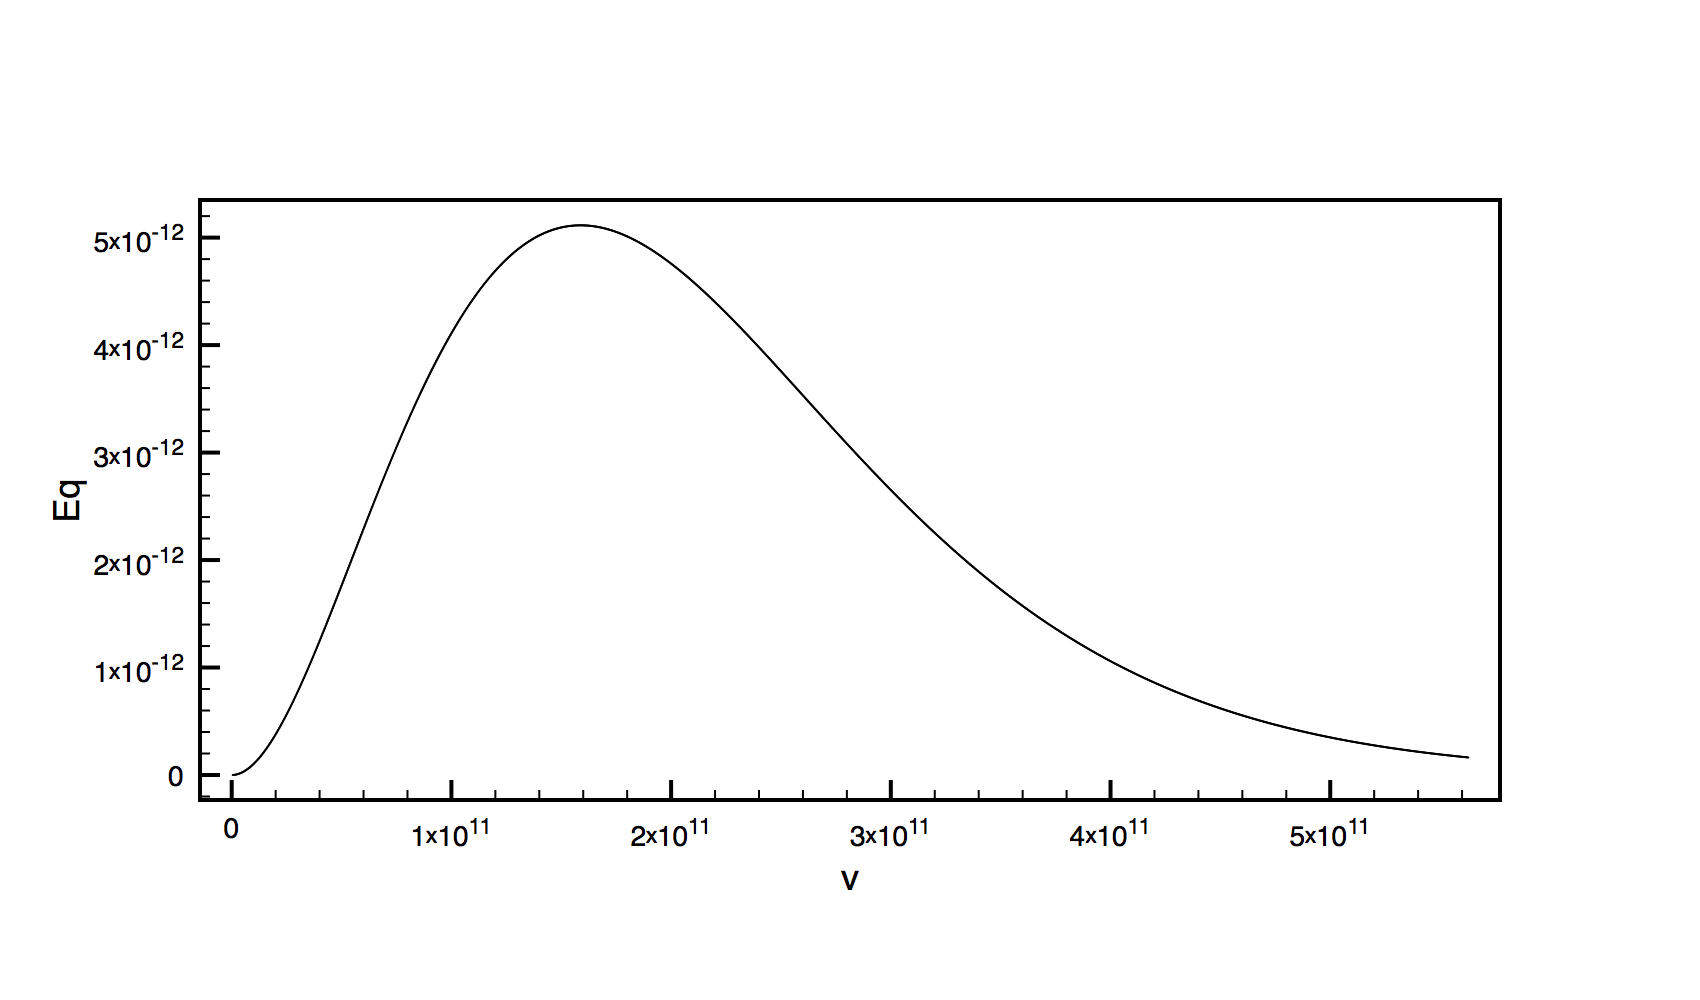
\includegraphics[width=1.\textwidth]{22.png}
	\caption{ V vs Eq at 300 Kelvin}
\end{figure}

\begin{figure}[H]
	\centering 
	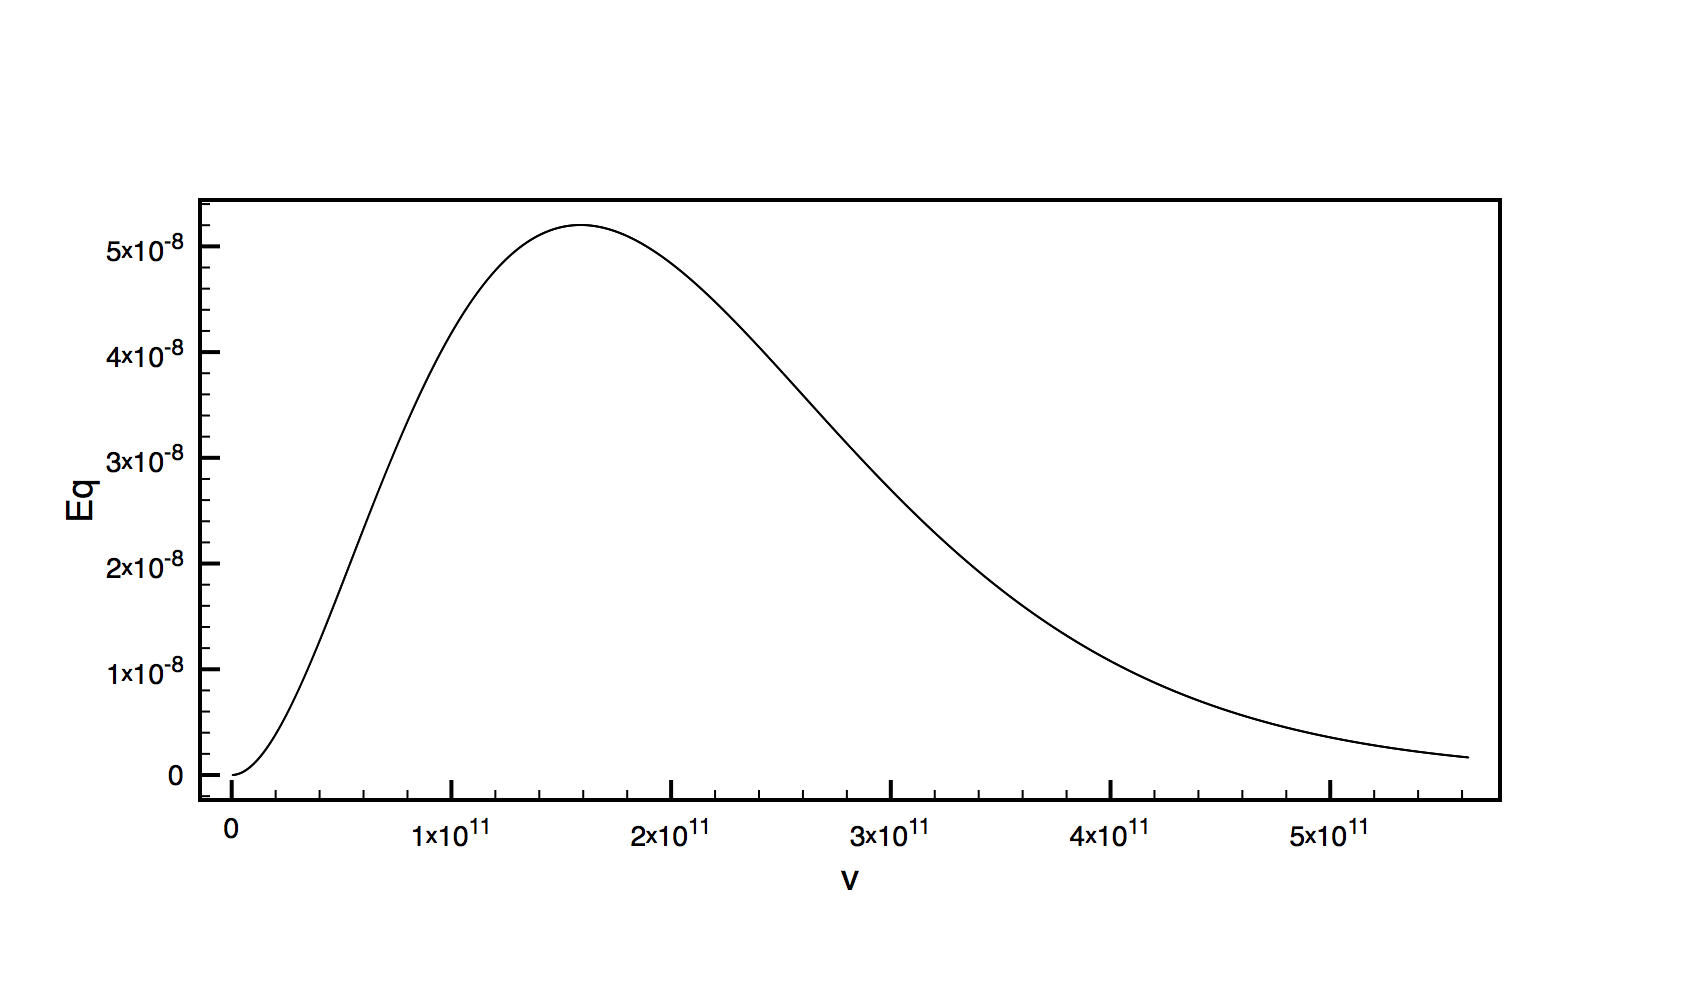
\includegraphics[width=1.\textwidth]{23.png}
	\caption{ V vs Eq at 6500 Kelvin}
\end{figure}


While all these graphs may be visually mysterious, but superimposing the curves can be help (7). As the spacing between each frequency is extremely large, a scaling factor was given to the the lower two temperatures to accommodate 2.7 K was scaled by ${}3*10^{10}{}$, and  300K by ${}1.5*10^{4}{}$. When applied, a trend forms with a raised vertex toward higher temperatures, signaling a corresponding release of higher frequencies.  


\begin{figure}[H]
	\centering 
	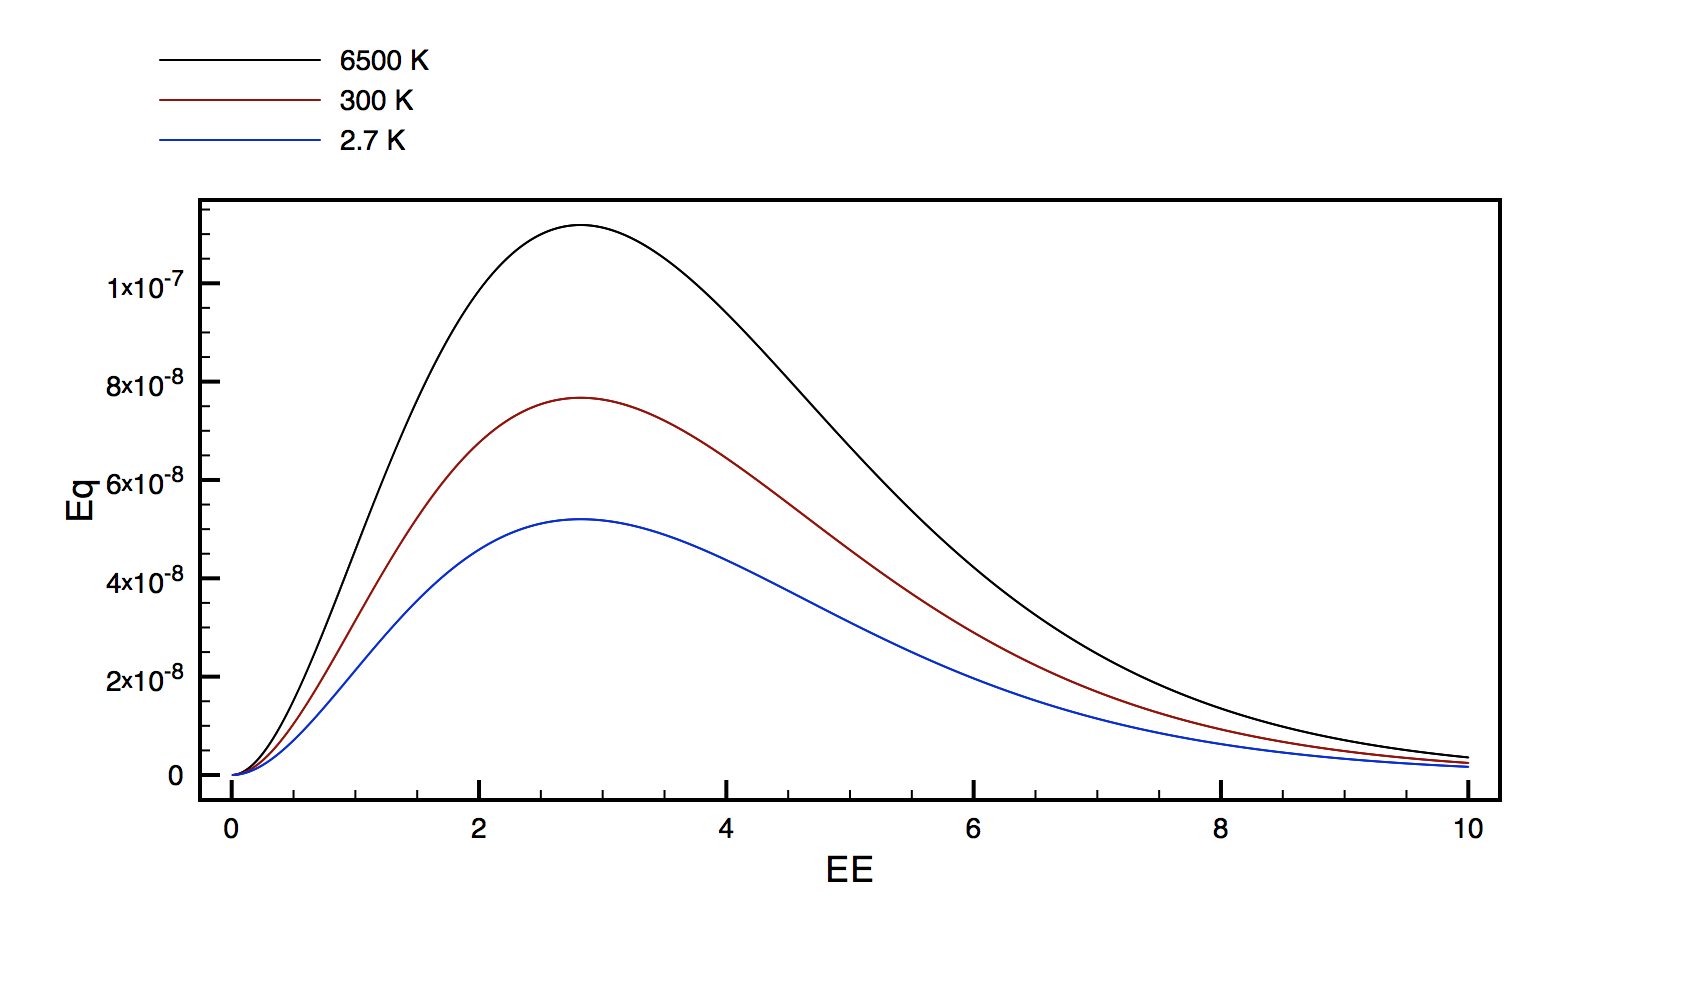
\includegraphics[width=1.\textwidth]{triple.png}
	\caption{Compiled graph of EE vs Eq}
\end{figure}



\section{Conclusions}

With respect to the modeling, consistency with the experimental data is needed, however with a trending vertex as well as a large deviation at the fixed temperature, we have fair amount of confidence in the results. This exploration helped define key steps for the future use in compiling mathematical code such as defining a dimensionless variable to be able to package the code for the output. Successive do loops and write statements, while repetitive creates easy step visualization for the reader to follow. With all this in place, we can finally give soon physical meaning to the programs output and in effect the problem, temperatures are held constant, of 2.7K 300K and 6500K, we have measurements of each respectively, in space, earth and the sun. The functions compile the radiance (electromagnetically) for an object in thermal equallibruim in each environment successfully.      


\begin{thebibliography}{}


\bibitem{metcalf} M.\ Metcalf, J.\ Reid and M.\ Cohen, {\it Fortran 95/2003 explained}. Oxford University Press, 2004.
 

\end{thebibliography}




\end{document}








